\documentclass{article}
\usepackage{listings}
\usepackage{xcolor}
\usepackage{graphicx}

\newcommand{\mytitle}[1]{
    \begin{center}
        {\LARGE #1} \\[0.5cm]
    \end{center}
}

% Define custom style for listings
\lstdefinestyle{mystyle}{
    backgroundcolor=\color{gray!10}, % Background color
    commentstyle=\color{green!50!black}, % Comment color
    keywordstyle=\color{blue}, % Keyword color
    numberstyle=\tiny\color{gray}, % Line number color
    stringstyle=\color{orange}, % String color
    basicstyle=\ttfamily\footnotesize,
    breakatwhitespace=false,
    breaklines=true, % enable line wrapping
    captionpos=b,
    keepspaces=true,
    numbers=left,
    numbersep=5pt,
    showspaces=false,
    showstringspaces=false,
    showtabs=false,
    tabsize=2
}

% Apply the custom style
\lstset{style=mystyle}

\begin{document}

\mytitle{2-SAT}

\lstinputlisting[language=C++]{../graph/2SAT.cpp}

\pagebreak

\mytitle{Bridge}

\lstinputlisting[language=C++]{../graph/bridge.cpp}

\pagebreak

\mytitle{Tarjan SCC}

\lstinputlisting[language=C++]{../graph/tarjan-scc.cpp}

\pagebreak

\mytitle{Convex Hull}

\lstinputlisting[language=C++]{../geometry/convex-hull.cpp}

\pagebreak

\mytitle{Line Segment Intersection}

\lstinputlisting[language=C++]{../geometry/line-segment-intersect.cpp}

\pagebreak

\mytitle{Dinic}

\lstinputlisting[language=C++]{../flow/Dinic.cpp}

\pagebreak

\mytitle{Max Matching}

\lstinputlisting[language=C++]{../flow/MaxMatching.cpp}

\pagebreak

\mytitle{MCMF}

\lstinputlisting[language=C++]{../flow/MCMF.cpp}

\pagebreak

\mytitle{BIT 2D}

\lstinputlisting[language=C++]{../data-structures/BIT2D.cpp}

\pagebreak

\mytitle{Dynamic CHT}

\lstinputlisting[language=C++]{../data-structures/dynamic-cht.cpp}

\pagebreak

\mytitle{Persistent Dynamic Segment Tree}

\lstinputlisting[language=C++]{../data-structures/persistent-dynamic-segment-tree.cpp}

\pagebreak

\mytitle{String Hash}

\lstinputlisting[language=C++]{../data-structures/string-hash.cpp}

\pagebreak

\mytitle{Treap}

\lstinputlisting[language=C++]{../data-structures/string-hash.cpp}

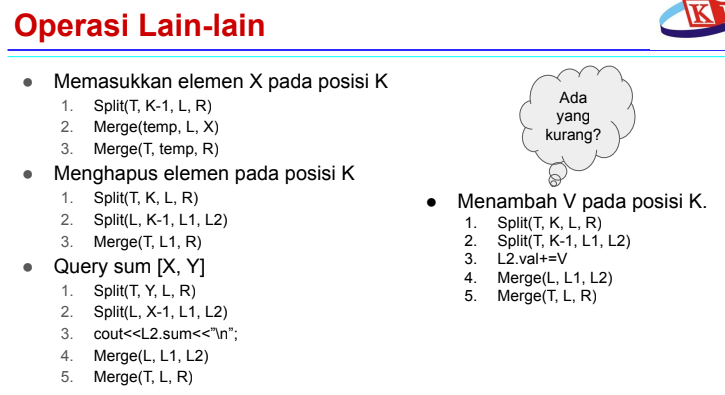
\includegraphics[width=0.8\linewidth]{../data-structures/treap-operations.png}

\pagebreak

\mytitle{PBDS}

\lstinputlisting[language=C++]{../data-structures/pbds.cpp}

\pagebreak

\mytitle{Matrix Mod Expo}

\lstinputlisting[language=C++]{../dynamic-programming/matrixmodexpo.cpp}

\pagebreak

\mytitle{Operator Overloading}

\lstinputlisting[language=C++]{../basic/operator-overloading.cpp}

\pagebreak

\mytitle{Li Chao Tree}

\lstinputlisting[language=C++]{../dynamic-programming/LiChaoTree.cpp}

\pagebreak

\mytitle{Dynamic Li Chao Tree}

\lstinputlisting[language=C++]{../dynamic-programming/DynamicLiChaoTree.cpp}

\pagebreak

\end{document}
